\part{Contributions}

\chapter{Traitement des données de mouvement}\label{chap:traitement_donnees}
Les chapitres précédents montrent que la capture de mouvement peu prendre place dans de nombreux contextes. Les besoins en termes d'observation et d'analyse peuvent varier grandement en fonction du domaine ciblé. Il est nécessaire de choisir un système de capture adapté, au regard des besoins d'observation mais également des contraintes de place, de coûts et de temps d'acquisition. De plus, il est nécessaire de disposer d'un ensemble d'outils logiciels afin de pouvoir extraire, à partir des données, des informations utiles pour l'apprentissage d'un geste. Ces informations peuvent être de plusieurs natures : il est possible de proposer une comparaison précise entre les données de l'expert et celles de l'apprenant (\textit{e.g.} " la position du coude est 4cm trop bas au moment $T$ du mouvement "), bien que cette méthode soit soumise aux problèmes de différences de morphologie, d'alignement temporel des séquences de mouvements, etc. Il est également possible de fournir des indications de plus haut-niveau (\textit{e.g.} " La vitesse lors du lancer doit être plus élevée "). Dans tous les cas, ces informations peuvent soit être utilisées telles quelles par l'apprenant, soit être utilisées par l'expert afin d'affiner son jugement du geste. Certaines conditions font qu'il n'est pas toujours possible pour un expert d'observer toutes les modalités importantes du geste pendant sa réalisation (trop de parties du corps à regarder, difficile de voir certaines parties du corps lors de l'exécution du geste, \textit{etc.}). La proposition d'outils d'aide à la décision permet ainsi d'aider l'expert dans sa tâche d'évaluation et de remédiation.

Ce chapitre présente l'artefact informatique développé pour répondre aux besoins de la thèse, nommé \textbf{Motion Learning Analytics} (\textbf{MLA}), ainsi que les différentes étapes du processus associé, du traitement des données de mouvements jusqu'à l'aide proposée à l'expert.

\section{Motion Learning Analytics (MLA)}
Dans cette partie, nous présentons la plateforme Motion Learning Analytics (MLA), créée pour répondre à nos besoins d'extraction et d'analyse de données de mouvement.

L'objectif de \textit{MLA} est de proposer un ensemble d'outils permettant d'extraire des informations permettant d'analyser un geste à partir de données de mouvement bas-niveaux, afin de pouvoir être utilisées par un humain \textit{a posteriori} afin d'aider au jugement de la qualité d'un geste en fonction du domaine applicatif. Il existe d'ores et déjà de nombreux systèmes d'analyse du mouvement. Ces systèmes ont déjà fait l'objet d'analyses. L'une d'entre elle propose une classification partielle selon l'objectif de ces systèmes \parencite{Wang2003Rdi} : la détection d'humains, le suivi (\textit{tracking}) d'humains et la reconnaissance d'activité. Bien que ces domaines soient larges et très explorés dans la littérature \parencite{Yang2011Raa} \parencite{Aggarwal2014Har}, ils concernent plutôt la segmentation et  l'extraction de mouvements au sein de différents types de données, tels que la vidéo ou des enregistrements partiels à l'aide de capteurs de parties du corps. De plus, le contexte applicatif est souvent secondaire et ces systèmes sont développés de manière à proposer des méthodes automatique innovantes. A l'inverse, notre approche se concentre sur une application particulière, celle de l'apprentissage du geste, afin de proposer des conseils à un apprenant ou à l'expert qui enseigne ce geste. De plus, l'objectif de notre système est d'être indépendant du geste considéré.

Des systèmes tels que ceux présentés dans le chapitre 2 (\parencite{Ferrari2018MAS}, \parencite{Makio2007DoS}) sont eux conçus pour une tâche ou un domaine en particulier. Le fait d'avoir un domaine ciblé dès le début permet d'orienter le développement et l'analyse afin d'offrir un retour à l'expert le plus exact possible. Le problème se pose dans la réutilisabilité de tels systèmes dans des cas proches : le système n'est pas systématiquement suffisamment modifiable pour être utilisé dans d'autres contextes. L'objectif de MLA est, à terme, de proposer un ensemble d'outils et de descripteurs calculables permettant de couvrir une large gamme de domaines applicatifs, à l'aide de l'injection de la connaissance de l'expert. Elle est divisée en trois parties : le traitement des données de mouvement brutes, de la lecture des fichiers jusqu'à l'extraction des descripteurs, l'analyse des données obtenues à l'aide de techniques d'apprentissage semi-supervisé, et le retour fourni à l'expert et/ou l'apprenant. Ces trois parties sont indépendantes l'une de l'autre, et peuvent être utilisées séparément. Chaque partie est découpée en modules, correspondant à un sous-ensemble de fonctions au sein de l'artefact. Le worklflow complet est présenté dans la figure  \ref{fig:workflow_MLA}.

\begin{figure}[h]
    \centering
    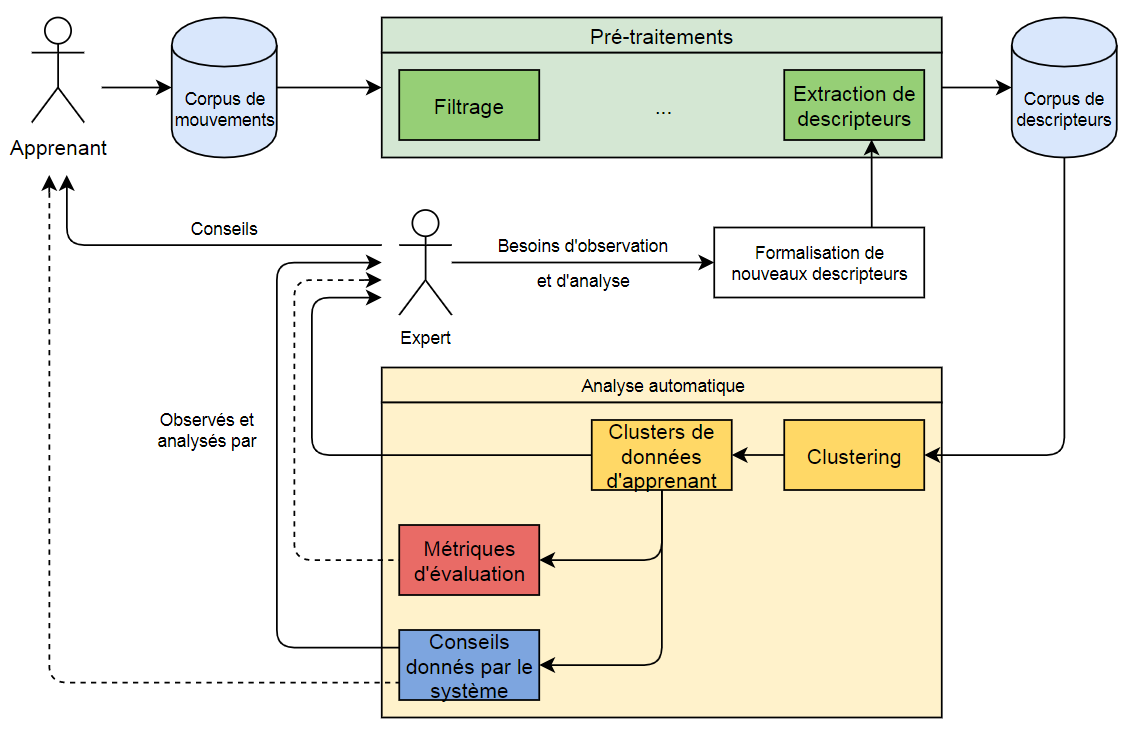
\includegraphics[width=\textwidth]{pictures/MLA_colours.png}
    \caption{Architecture de la plateforme \textit{Motion Learning Analytics} (\textit{MLA}).}
    \label{fig:mla_project}
\end{figure}

\begin{figure}[h]
    \centering
    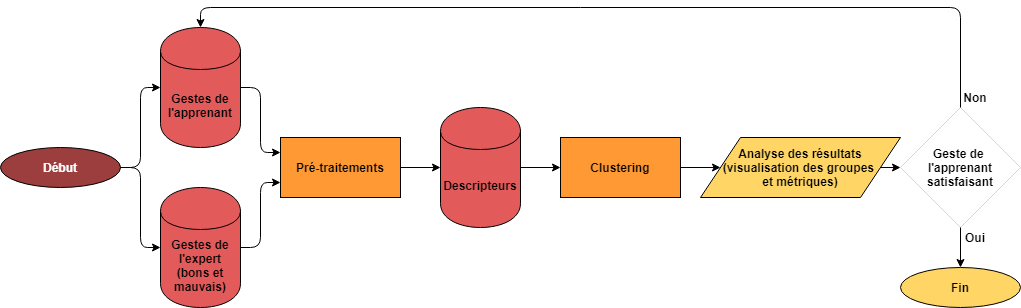
\includegraphics[width=\textwidth]{pictures/workflow_MLA_2.png}
    \caption{Le workflow général de la plateforme \textit{MLA}.}
    \label{fig:workflow_MLA}
\end{figure}

\subsection{Données de mouvement au format BVH}\label{subsec:bvh}
Le système prend en entrée des fichiers au format \textbf{BioVision Hierarchy} (\textbf{BVH}). Ce format de fichier permet de décrire un mouvement, posture par posture. Les fichiers \textbf{BVH} sont constitués d'une partie fournissant des informations sur les articulations composants le squelette, sous forme d'une hiérarchie (Fig. \ref{fig:bvh_hierarchy}), et d'une seconde partie donnant les informations pour chaque articulation sur chaque frame du mouvement (Fig. \ref{fig:bvh_motion}). Plus précisément, chaque articulation peut avoir jusqu'à six informations : trois valeurs relatives à la position dans l'espace, et trois valeurs relatives à l'orientation dans l'espace. Les informations pour chaque articulation sont données relativement à l'articulation parente.

\begin{figure}[h]
    \centering
    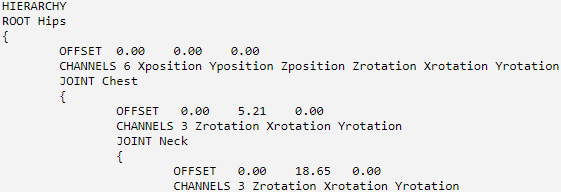
\includegraphics[width=\textwidth]{pictures/bvh_hierarchy.png}
    \caption[Exemple de squelette dans un fichier BVH]{Un exemple de la hiérarchie du squelette au sein d'un fichier BVH (source: \textit{http://research.cs.wisc.edu/graphics/Courses/cs-838-1999/Jeff/BVH.html})}
    \label{fig:bvh_hierarchy}
\end{figure}

\begin{figure}[h]
    \centering
    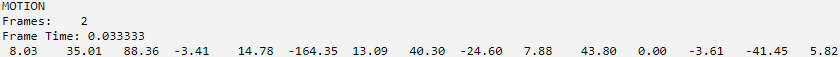
\includegraphics[width=\textwidth]{pictures/bvh_motion.png}
    \caption[Exemple de données de mouvement dans un fichier BVH]{Un exemple de données relatives au mouvement au sein d'un fichier BVH source: \textit{http://research.cs.wisc.edu/graphics/Courses/cs-838-1999/Jeff/BVH.html})}
    \label{fig:bvh_motion}
\end{figure}


\subsection{Pré-traitements des données}
La première partie (pré-traitements) a deux objectifs : (i) filtrer les données si nécessaire, afin d'éliminer les artefacts possibles dûs au matériel de captation, et (ii) extraire des descripteurs à partir du mouvement capturé, afin d'obtenir des informations exploitables. Cette partie est intégralement codée en \textbf{C++11}. Elle partie du système est subdivisée en six modules (Fig. \ref{fig:MLA_architecture}). Le module central de l'architecture contient les classes qui permettent de représenter un mouvement dans son entièreté, à partir d'un fichier \textbf{BVH}. La classe \textbf{Motion} contient les informations relatives au mouvement en général (nom du mouvement, nombre de frames, temps inter-frame, frame de référence), ainsi qu'une liste d'objets \textbf{Frame}. Cette classe représente une frame du mouvement et ne contient que des articulations : un pointeur vers l'articulation racine, et une liste d'objets de type \textbf{Joint} (\textit{articulation} en anglais). C'est à partir de l'objet \textbf{Motion} que les descripteurs sont extraits (Fig. \ref{fig:class_diagram_motion_MLA}). Une fois cette étape réalisée, les descripteurs sont insérés dans un objet de type \textbf{Data}, qui va ensuite pouvoir être exporté. Cet objet nécessite que les données aient (i) un nom, et aient la forme (ii) d'un vecteur contenant une liste de paires clés (le nom de l'articulation) / valeurs (la valeur du descripteur).


\begin{figure}[h]
    \centering
    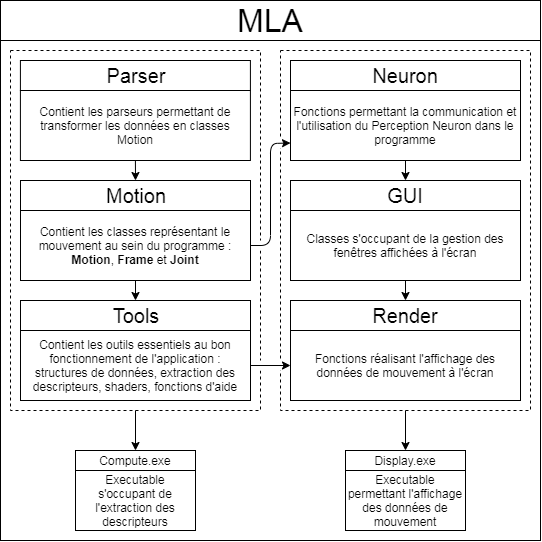
\includegraphics[width=\textwidth]{pictures/MLA_architecture.png}
    \caption[Architecture des pré-traitements et de l'affichage du mouvement capturé de \textit{MLA}]{L'architecture des pré-traitements et de l'affichage du mouvement capturé \textit{MLA}, divisée en six modules principaux.}
    \label{fig:MLA_architecture}
\end{figure}

\begin{figure}[h]
    \centering
    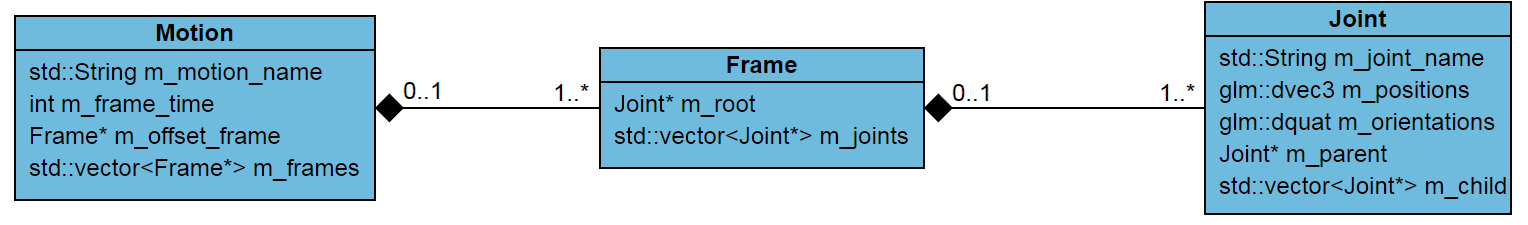
\includegraphics[width=\textwidth]{pictures/class_diagram_motion_MLA.png}
    \caption[Diagramme de classes du mouvement]{Diagramme de classes des trois classes composant le mouvement.}
    \label{fig:class_diagram_motion_MLA}
\end{figure}

Les descripteurs extraits du mouvement sont représentés au sein d'une structure \textbf{Data}, contenant le nom du descripteur, ainsi qu'un tableau contenant des couples de valeurs [nom de l'articulation] / [valeur du descripteur] (Fig. \ref{fig:class_diagram_datatype_MLA}). L'export de ces données se fait au format \textbf{JavaScript Object Notation} (\textbf{JSON}) (Fig. \ref{fig:json_data_example}), selon la hiérarchie suivante : descripteur $\rightarrow$ articulation $\rightarrow$ valeur. Le caractère peu-verbeux de ce format est un atout lors de l'export de fichiers de données volumineux. Sa très large utilisation, ainsi que le nombre conséquent d'analyseurs syntaxiques existants pour ce format en font un bon choix lorsque des données ont besoin de transiter d'une application à une autre \parencite{Gao2011JSON}. Il est ainsi possible de rechercher de manière naturelle (au sens du langage considéré) les descripteurs, en respectant le cheminement « descripteur $\rightarrow$ articulation ».

\begin{figure}[h]
    \centering
    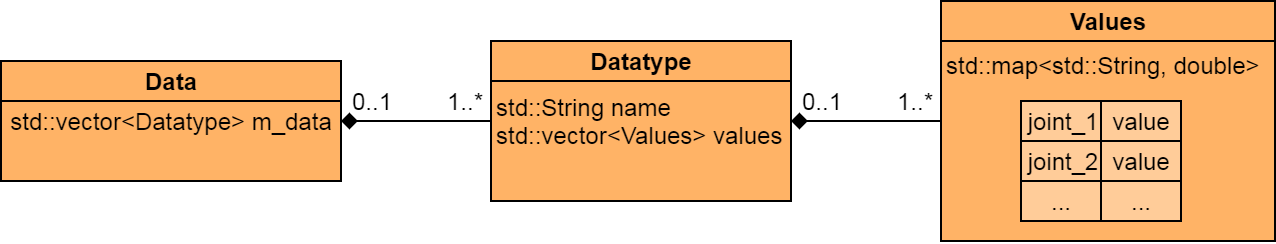
\includegraphics[width=\textwidth]{pictures/class_diagram_datatype_MLA.png}
    \caption[Diagramme de classes de la structure de stockage des données]{Diagramme de classes des classes composant la structure de stockage des données.}
    \label{fig:class_diagram_datatype_MLA}
\end{figure}

\begin{figure}[h]
	\centering
    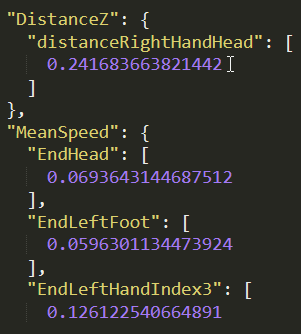
\includegraphics[]{pictures/json_data_example.png}
    \caption[Exemple de descripteurs au format JSON]{Un exemple de descripteurs extraits, au format JSON. Le stockage s'effectue selon la hiérarchie « descripteur $\rightarrow$ articulation $\rightarrow$ valeur ».}
    \label{fig:json_data_example}
\end{figure}

\subsection{Analyse automatique}
La partie Machine learning est codée en Python 3.6+. Le Python a été retenu comme langage pour le large choix de bibliothèques d'analyse de données et de machine learning.

L'objectif de cette partie est de proposer un ensemble d'outils permettant l'analyse des descripteurs extraits du mouvement capturé, à l'aide de techniques d'apprentissage non-supervisé. Il est possible de choisir un sous-ensemble d'articulations et de descripteurs à analyser à partir des données extraites, afin de concentrer l'analyse sur les parties du corps voulues. Un algorithme de \textit{clustering} est ensuite choisi, ainsi que les paramètres de cet algorithme. En fonction de l'algorithme, il est possible de modifier plusieurs paramètres : nombre de clusters (groupes) souhaités, taille du voisinage de recherche, \textit{etc.} Ce choix s'effectue pour l'instant par la personne gérant le programme, car le choix de l'algorithme et de ses paramètres doit se faire en fonction des données utilisées, et nécessite une connaissance scientifique. Des métriques sont ensuite calculées afin de fournir une indication quant à la qualité des regroupements obtenus. Il est possible de comparer les regroupements à un étiquetage des données, afin de vérifier si la séparation obtenue correspond aux \textit{a priori} de l'expert ou non. Cette phase de \textit{clustering} permet également d'obtenir deux groupes de mouvements : les mouvements cibles, et les mouvements avec défauts. Ces groupes sont ensuite utilisés pour donner un retour à l'apprenant.

\subsection{Feedback}
La partie feedback est également codée en Python 3.6+. L'objectif de cette partie du programme est de fournir un module proposant une aide à la décision pour un expert, mais également de proposer un retour compréhensible pour l'apprenant, dans le cas d'une utilisation sans expert. À partir de descripteurs pré-sélectionnés par l'expert lui-même, et d'exemples de mouvements réussis / ratés, le système fourni une aide visuelle afin de visualiser la différence entre les mouvements de l'expert et ceux de l'apprenant. L'objectif pour l'apprenant est de rapprocher le plus possible ses mouvements du groupe des mouvements cibles, en améliorant son geste au fur et à mesure de l'apprentissage, à l'aide des conseils dispensés par l'expert et/ou le système.\\


La plateforme MLA permet le traitement automatique de données de mouvement capturé, du filtrage au traitement automatique par des méthodes de \textit{clustering}, ainsi qu'à l'affichage synthétique d'information à destination de l'apprenant ou de l'expert. Cette partie a défini le contexte dans lequel s'incluent les travaux présentés dans cette thèse. Avoir une plateforme intégrant le traitement des données brutes, le calcul des descripteurs de mouvement, la comparaison et la visualisation des clusters de mouvements de l’apprenant possède l'avantage de centraliser les différentes étapes, et proposer ainsi un \textit{workflow} plus simple au sein d'un même artefact informatique. La suite de ce chapitre explique en détail le \textit{workflow} d'utilisation système.

\section{Capture de mouvement (Perception Neuron)}
Dans le cadre de cette thèse, la solution retenue pour la capture de mouvements a été celle de la combinaison de capteurs " Perception Neuron " \parencite{perceptionNeuron}, créée par l'entreprise NOITOM. Ce type de dispositif présente l'avantage d'offrir un compromis entre le coût et la qualité des données obtenues.

Le Perception Neuron est une combinaison de capteurs, basée sur l'utilisation de Neurons, des centrales inertielles (\textit{Inertial Measurement Unit}, ou \textbf{IMU} en anglais) composées d'un gyroscope, d'un accéléromètre et d'un magnétomètre. Ce type de capteur possède l'avantage d'être facilement portable par sa taille et son poids, et donc de présenter une gêne réduite pour l'utilisateur. Ces capteurs sont beaucoup utilisés dans le domaine médical \parencite{PORCIUNCULA2018S220}, pour l'analyse de la posture ou la rééducation d'une partie spécifique du corps par exemple.

Le Perception Neuron peut utiliser simultanément un ensemble de 32 Neurons au maximum. Les Neurons sont composés d'un accéléromètre, un gyroscope et un magnétomètre. Ces capteurs sont interchangeables, ce qui permet de ne changer que le Neuron défectueux si jamais un problème survient sur l'un d'entre eux. Cet ensemble de capteur est relié à un \textit{hub}, qu'il est possible de connecter à un ordinateur de manière filaire (liaison USB) ou non-filaire (WiFi). Le système est alimenté par un autre port USB, et il est possible d'utiliser une batterie USB rechargeable, afin d'obtenir une mobilité accrue. Il n'est possible d'utiliser le Perception Neuron que dans certaines configurations spécifiques (voir Fig. \ref{fig:perception_neuron_all_combinations}). Les données sont renvoyées à une cadence de 120 postures par secondes lorsque la combinaison est constituée de 17 Neurons ou moins, et de 60 postures par secondes lorsque le nombre de capteurs est supérieur ou égal à 18.

\begin{figure}
	\centering
    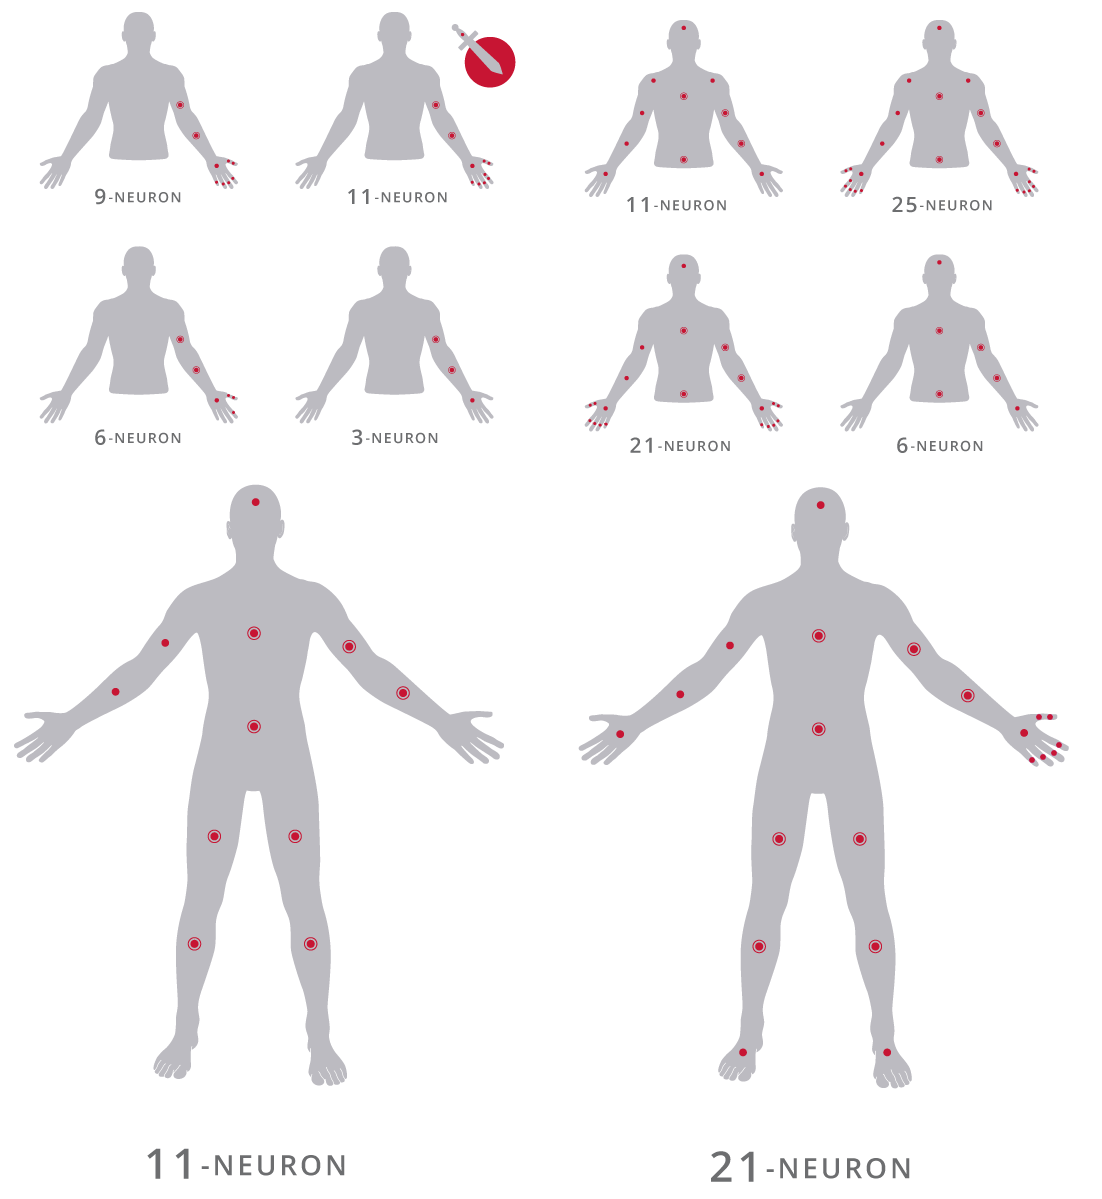
\includegraphics[width=\textwidth]{pictures/perception_neuron_all_combinations.png}
    \caption[Configurations possibles pour le Perception Neuron]{Toutes les configurations possibles pour le Perception Neuron \parencite{Noitom2015Doc}.}
    \label{fig:perception_neuron_all_combinations}
\end{figure}

Cette combinaison permet d'obtenir un squelette humain en 3D et donc d'éviter les problèmes propres aux  systèmes de capture vidéo 2D, en particulier celui de l'occlusion.

L'utilisation de cette combinaison nécessite l'utilisation du logiciel Axis Neuron, développé par NOITOM. Ce logiciel permet d'effectuer la communication entre le hub de la combinaison et l'ordinateur. Il est également le seul capable de lire le format de données dans lequel est enregistré le mouvement. Il permet de réaliser les calibrations de la combinaison, de visualiser en temps réel le mouvement réalisé, de rejouer un mouvement (avec possibilité de marche avant / marche arrière, ralentissement, etc.), d'utiliser différents squelettes afin de s'adapter à toutes les morphologies possibles, et d'éditer le mouvement.

\section{Pré-traitements des données}
Bien que présentant de nombreux avantages, les centrales à inertie ne sont cependant pas dénuées de problèmes \parencite{Giansanti2003Iif}. Le phénomène de la dérive (\textit{drift} en anglais) est le plus courant : il s'agit de l'accumulation d'erreurs d'intégration, qui sert à obtenir l'information d'orientation de position à un temps $T$ à partir de la vitesse, elle-même déduite de l'accélération. Les capteurs magnétiques sont également sensibles aux perturbations extérieures : la présence d'objets métalliques, ou d'objet émettant un champ électromagnétique. Ces phénomènes combinés font que les données obtenues lors des captures de mouvements ne sont pas toujours précises. La différence entre le geste réalisé par une personne et le geste visualisé sur le logiciel Axis Neuron est parfois très grande. De plus, le logiciel Axis Neuron applique des traitements aux données reçues des capteurs. Ils sont au nombre de trois : \textit{Embeded Data Fusion}, \textit{Human Body Dynamics} et \textit{Physical Engine}. Ces algorithmes sont propriétaires, et donc non documentés de manière exhaustive : il est très difficile de savoir dans quelle mesure les données sont modifiées avant d'être présentées dans le logiciel. À cause de cette limitation, des corrections de données ont été effectuées sur les descripteurs extraits du mouvement, et non sur le mouvement original lui-même. Dans les parties suivantes, nous traitons des signaux. Le terme \textit{artefacts} sera ici utilisé pour décrire les erreurs présentes au sein de ces signaux, dues au matériel de capture, et non pour parler d'un artefact informatique.

\section{Traitements des données de mouvement}\label{sec:traitements}
Dans le cadre de tests du système, des mouvements de lancers ont été utilisés afin d'en extraire des descripteurs. Ces descripteurs était relatifs aux vitesses de la main. Un des premiers tests du système a été la vérification de la cohérence de ces descripteurs par rapport au mouvement réel. Lors de l'extraction d'informations à partir des données de mouvement, il a été remarqué que les vitesses extraites à partir des positions successives présentaient des \textit{artefacts} conséquents (Fig. \ref{fig:linear_speed_artifacts}). Ces \textit{artefacts} se retrouvent le plus souvent lorsque des changements brusques de vitesse se produisent, c'est-à-dire quand l'accélération augmente ou décroit rapidement. Il n'est pas possible d'utiliser des données présentant ces défauts sans une étape de correction. L'analyse de l'origine de ces \textit{artefacts} a permis de mettre au jour deux problèmes majeurs des données de mouvement provenant du logiciel Axis Neuron : le changement de la taille des membres du squelette au cours du temps, et les problèmes d'incohérences de changement de position d'une frame à une autre.

\begin{figure}
	\centering
    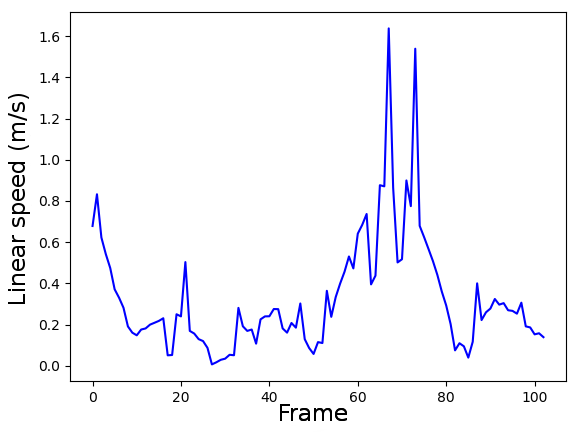
\includegraphics[width=7.5cm]{pictures/linear_speed_artifacts.png}
    \caption[Vitesse linéaire avec artéfacts]{Un exemple de vitesse linéaire extraite d'un mouvement. On remarque bien les pics de vitesse (autant vers le haut que vers le bas) entre les frames 60 et 80 (abscisses), ne correspondant pas à un lancer fluide.}
    \label{fig:linear_speed_artifacts}
\end{figure}

\subsection{Variation de la taille des membres}
Un des premiers problèmes rencontrés a été la variation de la taille des membres du corps au cours du mouvement. Il apparaît que la taille des membres ne reste pas fixe tout au long du lancer. Ce problème peut provenir soit de l'imprécision des capteurs, soit des traitements effectués avant la restitution du mouvement.

Une solution simple est de fixer cette taille, qui correspond à l'écartement entre les articulations, pour chaque membre. Pour chaque enregistrement, il existe une posture de référence, qui contient toutes les informations de position et d'orientation pour chaque articulation. Cette \textit{frame} est créée après la phase de calibration, ce qui fait qu'elle est moins sujette aux problèmes inhérents aux capteurs, car ces derniers surviennent au bout d'un certain temps de captation.

Pour chaque articulation, les informations sont stockées sous la forme d'un vecteur de dimension 3, correspondants aux positions de l'articulation en $x, y, z$, et d'un quaternion correspondant à la rotation de cette articulation. Ces informations sont données par rapport à l'articulation parente : les valeurs de position et d'orientation d'une articulation fille $j_{i+1}$ sont donc données relativement à l'articulation mère $j_i$, et la position de l'articulation fille $p_{j_{i+1}}$ correspond donc à la taille du membre $m_{j, j+1}$. La première étape du traitement des données par la plateforme MLA consiste donc à copier les positions de l'articulation de la frame de référence sur toutes les autres frames du mouvement. L'orientation reste inchangée.

\subsection{Incohérences de position des articulations d'une frame à une autre}

Un autre défaut présent dans les données a été constaté lorsque les vitesses ont été extraites des mouvements. Dans le cadre de tests, un mouvement de lancer a été enregistré, afin d'en extraire des descripteurs. Il s'est avéré que les valeurs de vitesses pouvaient parfois varier grandement d'une \textit{frame} à une autre, sans pour autant que cette variation ne soit représentative du mouvement réel (Fig. \ref{fig:linear_speed_artifacts}). En effet, lors du lancer test, et après observation de l'enregistrement vidéo correspondant à ce lancer, il apparaît que les variations de vitesses très brèves (correspondantes aux pics vers le haut et vers le bas du signal) ne correspondaient pas à la réalité du mouvement. À l'œil nu, lorsque le mouvement est affiché à l'écran, ces erreurs ne sont pas visibles, car ces variations apparaissent sur des temps très courts (de l'ordre du centième ou du millième de seconde). Cependant, lors de l'extraction de la vitesse, il apparaît que la variation est parfois extrême sur un ensemble de frames données.

Nous avons formulé quatre hypothèses pour expliquer ces incohérences de non-linéarité dans le mouvement :
\begin{enumerate}
	\item Le pas de temps entre les \textit{frames} est constant, et l'interpolation entre ces \textit{frames} est incorrecte, ce qui signifie que l'implémentation de l'interpolation entre les \textit{frames} est mal réalisée au sein du logiciel Axis Neuron.
	\item Le pas de temps entre les \textit{frames} est constant, et il n'y a pas d'interpolation, ce qui signifie qu'il manque des \textit{frames}. Ce problème pourrait subvenir lorsque la combinaison n'arrive pas à retourner les données des capteurs, à cause du trop grand nombre de données à traiter en simultané et en temps réel.
	\item Le pas de temps entre les \textit{frames} n'est pas constant et il y a interpolation, ce qui signifie que l'interpolation est incorrecte à cause d'un mauvais indice temporel donné à la \textit{frame} reconstituée. Supposons un mouvement linéaire composé de trois frames $f_0, f_2, f_4$ prises aux temps $t_0, t_{0+2}, t_{0+4}$ respectivement. Si le système ne renvoie que les informations des frames $f_0$ et $f_4$, l'interpolation entre la première frame $f_0$ et la deuxième frame $f_4$ reçue, étant supposée correspondre à l'instant $t_{0+1}$, correspondra en fait au moment $t_{0+2}$.
	\item Le pas de temps entre les frames n'est pas constant, et il n'y a pas d'interpolation, ce qui signifie qu'il manque des frames. Supposons un mouvement linéaire composé de cinq frames $f_0, f_1, f_2, f_3, f_4$ prises aux temps $t_0, t_{0+1}, t_{0+2}, t_{0+3}, t_{0+4}$ respectivement. Si le système ne renvoie que les informations des frames $f_0$, $f_1$, $f_3$ et $f_4$, il y aura un déplacement entre les frames $f_1$ et $f_3$ correspondant à $2*t$.
\end{enumerate}

Le tableau \ref{linear_speed_problem_hypothesis_table} résume ces hypothèses.
\begin{center}
\begin{table}[h!]
\begin{tabular}{l|l|l}
& \makecell{Interpolation} & Pas d'interpolation \\\hline
\makecell{Intervalle de temps\\constant} & \makecell{Mauvaise interpolation} & \textit{Frames} manquantes                  \\\hline
\makecell{Intervalle de temps\\non-constant} & \makecell{Mauvaise posture\\dû a un indice temporel erroné} & \makecell{\textit{Frames} affichées\\au mauvais moment}
\end{tabular}
\caption{Résumé des hypothèses sur les incohérences de positions}
\label{linear_speed_problem_hypothesis_table}
\end{table}
\end{center}

Il est possible que ces erreurs proviennt d'une baisse de la fréquence de retour des donneés, ou d'un problème d'acquisition des capteurs. En effet, sur le logiciel Axis Neuron®, chaque capteur possède un indicateur visuel permettant de juger de la qualité des données retournées : vert (OK), jaune (moyen), rouge (mauvais). Il n'existe cependant aucune indication sur la nature des dégradations des données. Indépendament de la cause, il est possible de proposer des solutions permettant de pallier ce problème. Ces constatations font qu'il était nécessaire de trouver une manière de nettoyer les données avant leur utilisation. Plusieurs pistes ont été évoquées. Il serait possible de reconstruire le mouvement par interpolation, avec un pas de temps fixe. En prenant un pas de temps suffisamment grand, on peut espérer obtenir un mouvement recomposé évitant les sauts de distance. Cependant, en faisant ainsi, le nombre de \textit{frames} du mouvement recomposé sera bas, et le mouvement recomposé risque de passer outre des moments clés du mouvement original (flexion d'une partie du corps, variation de l'accélération, etc.). Il existe des techniques d'interpolation se basant sur des \textit{frames} clés (\textit{key-frames}), afin de garder les informations cruciales du mouvement \parencite{Brotman1988MIO}. Cette méthode nécessite de définir ces \textit{frames} clés à l'avance. Or, au vu du nombre de données à traiter, il est difficile de spécifier manuellement ces frames clés pour chaque mouvement enregistré.

Les descripteurs vitesses extraits à partir du mouvement originel présentaient donc des \textit{artefacts}. De par les caractéristiques propres à ces \textit{artefacts} (pics très intenses et de courte durée), un filtre a été appliqué sur les valeurs de vitesses ainsi obtenues. Cette étape est cruciale, car les valeurs de vitesses sont utilisées plus tard dans la chaine de traitement afin de segmenter le mouvement.

Il existe plusieurs types de filtres pouvant être appliqué à un signal, afin d'en réduire le bruit. Rojas-Lertxundi \textit{et al.} présentent plusieurs de ces filtres dans \parencite{Rojas2015MCS}. Parmi eux, le filtre passe-bas a été utilisé par Kristianslund \textit{et al.} \parencite{KRISTIANSLUND2012Eol} afin de filtrer les signaux provenant des mouvements des articulations de joueurs de handball et d'améliorer la détection et la prévention de blessures. Le filtre de Butterworth est un filtre qui possède un gain constant dans sa bande passante. Il a été utilisé par Malfait \textit{et al.} \parencite{Malfait2014Hra} afin de filtrer des données de test de détente. Les filtres de Chebyshev sont des filtres qui proposent une plus grande ondulation soit en bande passante (Type I) soit en bande atténuée (Type II) que les filtres de Butterworth. Il a été utilisé par Fanis et Stathis \parencite{Moschas2011Mot} afin de réduire le bruit provenant de données GPS et d'accéléromètre. Le filtre de Kalman repose sur le principe de l'estimation de données à partir de l'observation de données bruitées. Ces filtres sont très utilisés pour filtrer les données provenants d'IMUs \parencite{Zihajehzadeh2014Act} \parencite{Marins2001AeK} \parencite{Luinge1999Eow}. Le filtre de Savitsky-Golay est un filtre passe-bas servant à lisser une courbe \parencite{Savitsky1964SaD}. Il se base sur une fenêtre glissante, et effectue une régression afin de déterminer le polynôme minimisant l'erreur au sens des moindres-carrés pour un point donné. Plus cette fenêtre est large, plus le signal sera lisse, et plus les pics courts seront atténués. Le degré de ce polynôme dépend du cas applicatif : un polynôme de degré 2 permet de prendre en compte une courbure dans le signal, alors qu'un polynôme de degré 3 permet de prendre en compte les points d'inflexion du signal.

Ce filtre a été retenu, de par sa simplicité de compréhension, sa rapidité d'exécution et également son principe de réduction du bruit (à l'inverse du filtre Kalman, qui lui trouve des informations au sein d'un signal bruité). De plus, bien que le filtre de Kalman semble être un candidat judicieux au vu du matériel utilisé, il est habituellement utilisé pour traiter les données de mouvement provenant directement des capteurs, et non les descripteurs extraits de ces derniers.

La détermination des paramètres de ce filtre s'est effectuée de manière empirique. La taille de la fenêtre symétrique correspond à $\frac{T}{4}$, avec $T$ étant la durée totale de l'enregistrement du mouvement. Le polynôme utilisé est de degré $3$ : une valeur inférieure lisse trop les données, et résulte en une perte d'information, alors qu'une valeur supérieure créée un sur-ajustement \ref{savgol_comparison_all_3_at_once}. Il a été déterminé empiriquement qu'une taille de fenêtre de $ \frac{nbframes}{4}$ permettait d'obtenir un signal lissé, sans pour autant en gommer les caractéristiques principales.

\begin{figure}
	\centering
    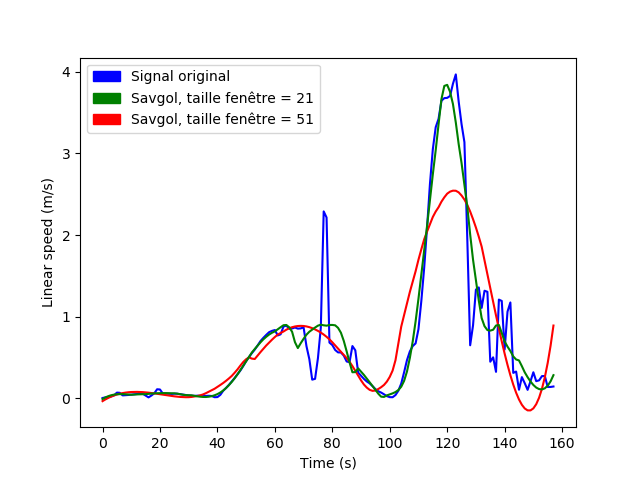
\includegraphics[width=\textwidth]{pictures/savgol_comparison_all_3_at_once.png}
    \caption[Comparaison de l'influence des paramètres d'un filtre Savitsky-Golay]{Un exemple de filtrage de données de vitesses par un filtre de Savitsky-Golay. Le signal original est en bleu, suivit par les résultats du filtrage avec une taille de fenêtre de 21 en vert) et une taille de fenêtre de 51 (en rouge). Une taille de fenêtre trop élevée efface tous les artefacts présents, mais gomme également les caractéristiques propres du signal (le changement brusque de vitesse).}
    \label{savgol_comparison_all_3_at_once}
\end{figure}

L'application de ce filtre sur les données de vitesse bruités (Fig. \ref{fig:before_after_savgol}) permet d'obtenir une courbe plus lisse, se rapprochant d'avantage de la réalité de la vitesse du mouvement effectué. La courbe de vitesse lors du lancer correspond aux enregistrements, et il est également possible de distinguer les gestes d'amplitude plus faible précédent le lancer (dans le cas présent, il s'agit de l'étape de balancement de la main avant le lancer, voir Fig. \ref{fig:after_savgol_explained}).

\begin{figure}
	\centering
    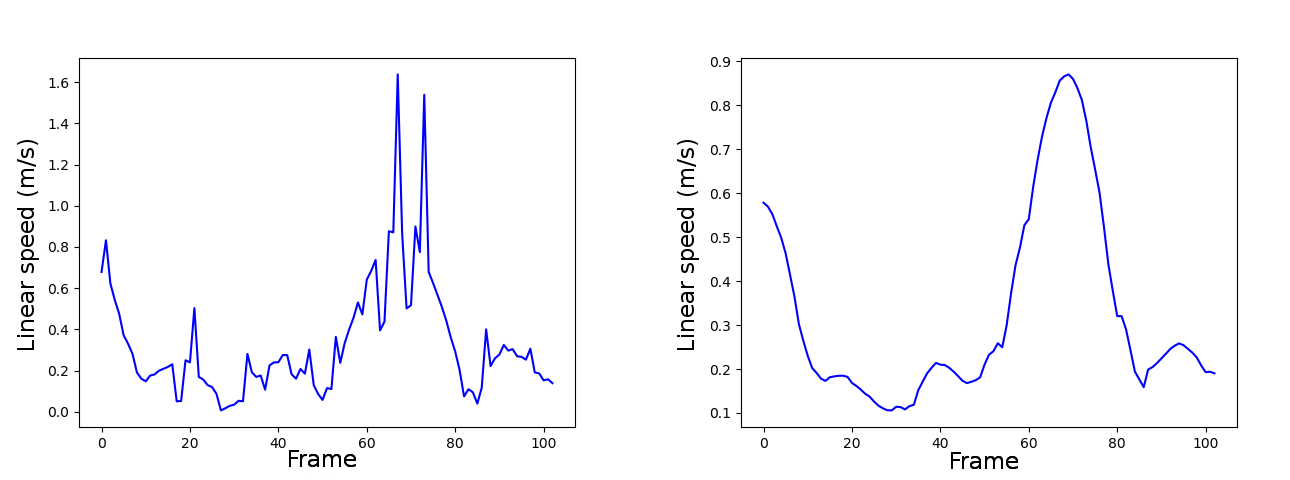
\includegraphics[width=\textwidth]{pictures/before_after_savgol.png}
    \caption[Vitesses filtrées par un filtre de Savitsky-Golay]{Un exemple de vitesse linéaire filtrée (à droite) à l'aide d'un Savitsky-Golay. Les pics correspondants aux artefacts du mouvement on disparu, et les caractéristiques initiale du changement de vitesses ont été conservées.}
    \label{fig:before_after_savgol}
\end{figure}

\subsection{Extraction du moment d'intérêt du mouvement}\label{subsec:MoI}
Lors de l'analyse d'un mouvement, il n'est pas systématiquement nécessaire de disposer de l'intégralité du mouvement. Par exemple, dans le cadre d'un service au tennis, l'analyse du mouvement se concentre sur les parties hautes du corps, notamment le poignet de la main qui tient la raquette \parencite{Makio2007DoS}. Il est également possible que le mouvement jugé utile soit contenu au sein d'un enregistrement plus large : il faut alors être capable d'extraire le mouvement d'intérêt. Segmenter manuellement un mouvement est une tâche réalisable par un humain. Cependant, en fonction du nombre de données à traiter, de la durée totale des mouvements, du nombre de passages à segmenter, cette tâche peut devenir chronophage. La segmentation automatique du mouvement peut pallier ce problème.

Il existe plusieurs techniques de segmentation automatique du mouvement \parencite{Zappella2008MSR}. L'ensemble des techniques permettant cette segmentation se basent sur différentes méthodes : apprentissage supervisé / non-supervisé, réduction de dimension, etc. Le choix de la méthode se base souvent sur la connaissance \textit{a-priori} des caractéristiques propres au mouvement. Les techniques à base d'apprentissage supervisé supposent que les classes (\textit{i.e.} les types de mouvements présents au sein du corpus) soient connues en amont. À l'inverse, les techniques non-supervisées ne possèdent pas d'\textit{a-priori} sur le type du mouvement : la segmentation se fait sans assignation à une classe.

Les méthodes de segmentation à base d'apprentissage supervisé se basent sur un corpus d'apprentissage correspondant au sous-mouvement à extraire du mouvement principal. Ces méthodes proposent souvent à la fois une segmentation en actions et une classification de ces actions. En entrainant des classifieurs sur des séquences choisies avec soin au préalable, il est possible d'obtenir une segmentation du mouvement, en fonction des différentes actions présentes. Les méthodes peuvent faire appel à des classifieurs SVM \parencite{Hoai2011Seg}, des modèles de markov cachés (\textit{Hidden Markov Models}, \textit{HMM}) et une combinaison de classifieurs faibles afin de créer un classifieur fort (Multi-class Adaboost) \parencite{Fengjun2006Ada}, ou encore des réseaux de neurones \parencite{Bouchard2007SSM}. Ces méthodes nécessitent toutes un corpus préalablement constitué, étiqueté et sont le plus souvent testées sur des corpus de mouvements existants et connus, tels que CMU \parencite{CMUDatabase} et HDM05 \parencite{HDM05Database}. Ces bases sont constituées de nombreux mouvements, tels que se lever, s'asseoir, prendre un objet, etc. Ces mouvements ne nécessitent pas d'effort cognitif particulier pour un humain, et donc ne sont pas sujet à un quelconque apprentissage. De plus, lorsque le domaine métier ne dispose pas de base de mouvements pré-établie, il faut en constituer une en disposant de suffisamment d'exemples étiquetés, et couvrant une grande variété de cas (différences de morphologie, de durée, de manière de faire, etc.).

La segmentation de mouvement par l'approche à base d'apprentissage non-supervisé permet de s'affranchir de certaines de ces contraintes. L'objectif reste le même, à savoir décomposer un mouvement en plusieurs sous-mouvements, mais cette fois sans \textit{a-priori} sur ces séparations. Trois méthodes ont été proposées par Barbi \textit{et al.} \parencite{Barbic2004SMC}, traitant toutes le mouvement comme étant une séquence ordonnée de \textit{frames}. A partir des données de rotation (quaternions), une analyse en composantes principales (\textit{PCA}) de ces données est réalisée sur chaque \textit{frame}, afin d'obtenir une représentation de plus basse dimensionnalité. Cette approche se base sur le fait qu'un mouvement simple aura une représentation de basse dimensionnalité. En minimisant l'erreur de projection, la dimensionnalité optimale est trouvée. En calculant ensuite la dérivée des valeurs succesives de l'erreur, il est possible de détecter les fractures au sein du mouvement, \textit{i.e.} là où la dérivée augmente fortement. La deuxième méthode se base sur l'analyse en composantes principales probabilistes (\textit{PPCA}) \parencite{Tipping1999PPCA}. Les premières \textit{frames} du mouvement sont modélisées sous forme d'une distribution Gaussienne, en fonction de la dimension intrinsèque estimée. La probabilité d'appartenance des \textit{frames} suivantes à la distribution Gaussienne est ensuite calculée, à l'aide d'une distance de Mahalanobis. En augmentant progressivement le nombre de frames utilisées pour le calcul de la distribution Gaussienne, il est possible d'obtenir une courbe de la distance calculée à chaque fois. Les pics de cette courbe apparaissent lorsqu'un changement de comportement survient : il s'agit du moment où le mouvement change, et donc où la segmentation va prendre place. La dernière technique proposée dans ces travaux se base sur un modèle de mélange de gaussiennes (\textit{GMM}). L'hypothèse de départ est que les frames de différents mouvements simples vont former différents clusters. Le PCA est utilisé afin de réduire les temps de traitements de l'algorithme d'estimation, et le nombre de composantes à garder est choisi afin que $90\%$ de la variance de la distribution des données originale soit préservée. Une fois les paramètres du modèle estimés, un cluster d'appartenance est calculé pour chaque \textit{frame}. L'inconvénient de cette méthode est qu'il faut spécifier à l'avance le nombre de clusters.

Une autre technique utilise l'analyse de clusters alignés, afin d'obtenir une segmentation du mouvement \parencite{Zhou2008ACA}. Cette méthode réduit le problème de la segmentation à un problème de \textit{clustering}. Elle est basée sur l'algorithme des \textit{k-means}, et propose deux changements majeurs par rapport à cet algorithme : la taille des caractéristiques d'un cluster peut varier, et la fonction de distance utilisée se base sur la déformation temporelle dynamique (\textit{DTW}). Cette technique permet de calculer une similarité entre deux séries temporelles, tout en étant robustes aux décalages de phase sur l'axe du temps \parencite{Berndt1994DTW}. Afin d'appliquer cette segmentation à de larges corpus, il est nécessaire d'opérer une réduction du nombre de \textit{frames} initiales.

La granularité de la décomposition peut grandement varier. Ainsi, la méthode développée par Krüger \textit{et al.} \parencite{Kruger2017EUT}, en utilisant en premier lieu du regroupement de caractéristiques, puis ensuite le voisinage des graphes constitués par les caractéristiques propres à chaque \textit{frame}, permet non seulement de séparer différentes actions au sein d'un mouvement initial (par exemple, une personne qui marche puis qui se met à courir), mais également de subdiviser encore les sous-mouvements obtenus en primitives (par exemple, les pas individuel lors de la marche et de la course).

%La segmentation obtenue est souvent dénuée de sémantique, bien que des études permettent d'obtenir dans un premier temps la segmentation, puis dans un deuxième temps de relier cette division à des étiquettes

Bien que les techniques précédemment présentées atteignent des bons taux de segmentation (par rapport à la segmentation manuelle), la solution retenue est plus simple, et se base sur les pics de vitesses du mouvement. Cet algorithme permet une segmentation rapide des mouvements, dès lors que le mouvement d'intérêt présente une forte variation de vitesse. Les mouvements caractéristiques des expérimentations sont le passage d'une vitesse quasi-nulle (position stationnaire), ou d'une vitesse faible (mouvement de balancier avant le lancer), a une vitesse élevée (mouvement du lancer), puis au retour à une vitesse faible, voire nulle (position de repos). La solution retenue permet ainsi une bonne segmentation du mouvement d'intérêt (\textit{Motion of Interest}, \textit{MoI}). L'algorithme de segmentation qui a été développé se base sur un repérage de la valeur maximale de la vitesse d'une articulation pré-déterminée. Dans le cas d'étude présenté, la main est l'articulation choisie, car nous nous plaçons dans le cas de mouvements de lancer, et cette articulation est source de la plus grande amplitude en terme de positions. Il serait cependant possible de déterminer automatiquement quelle articulation présente la plus grande amplitude de variations de vitesses, et de trouver ainsi le pic de vitesse maximale lors du geste. En partant de ce maximum, la segmentation s'effectue en choisissant un nombre de minimum locaux à franchir avant et après ce maximum. Ce choix permet d'intégrer au \textit{MoI} les phases de balancement pré-lancer, par exemple. Dans notre cas, nous nous limitons au \textit{MoI} seul. L'algorithme ainsi choisi (Algorithm \ref{algorithm_MoI}) permet de limiter la consommation de ressources (temps et mémoire).

\begin{algorithm}
\caption{MoI extraction algorithm}
\begin{algorithmic}[1]
\State $motion$: the full motion
\State $lc$: the number of desired left cuts
\State $rc$: the number of desired right cuts
\Procedure{Motion segmentation}{$motion$, $lc$, $rc$}
	\State $hs \gets$ GetHighestSpeedValue($motion$)
    \State $p\_lm \gets$ GetPreviousLocalMin($hs$)
    \State $n\_lm \gets$ GetNextLocalMin($hs$)
    \State $left\_found$ = 0
    \State $right\_found$ = 0
    \State $seg\_motion \gets$ segmented motion from $p\_lm$ to $n\_lm$
 	\While{$left\_found$ < $lc$}
          \State $n\_lm$ = $p\_lm$
          \State $p\_lm \gets$ GetPreviousLocalMin($p\_lm$)
          \State $seg\_motion \gets$ $motion$ from $p\_lm$ to $n\_lm$ added at the beginning
  	\EndWhile

    \While{$right\_found$ < $rc$}
          \State $p\_lm$ = $n\_lm$
          \State $n\_lm \gets$ GetNextLocalMin($n\_lm$)
          \State $seg\_motion \gets$ $motion$ from $p\_lm$ to $n\_lm$ added at the end
  	\EndWhile

 \EndProcedure
 \end{algorithmic}
 \label{algorithm_MoI}
\end{algorithm}

\begin{figure}
	\centering
    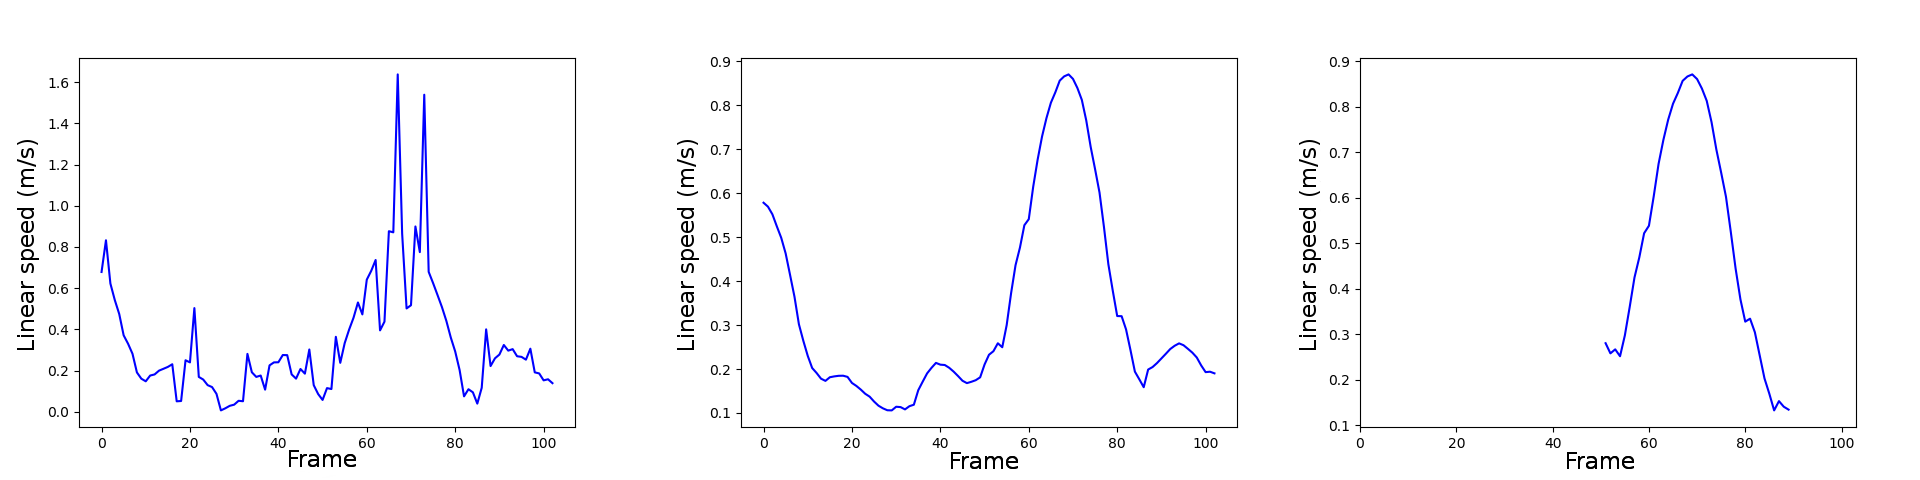
\includegraphics[width=\textwidth]{pictures/speed_values_all.png}
    \caption[Vitesse linéaire filtrée et segmentée]{Un exemple de vitesse linéaire filtrée puis segmenté par l'algorithme \ref{algorithm_MoI}.}
    \label{fig:speed_values_all}
\end{figure}

Cette étape marque la fin de la chaîne de pré-traitement des données de mouvement. En sortie de cette chaîne, un mouvement filtré et segmenté est proposé, afin de n'extraire les descripteurs que des parties d'intérêt du mouvement (Fig. \ref{fig:speed_values_all} et \ref{fig:after_savgol_explained}).

\begin{figure}
	\centering
    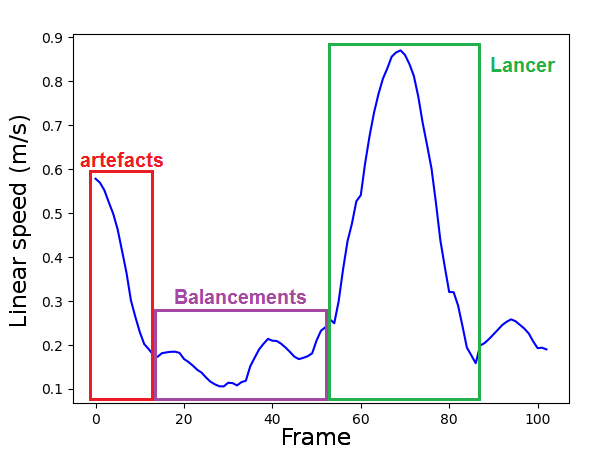
\includegraphics[width=10cm]{pictures/after_savgol_explained.png}
    \caption[Signal filtré décomposé en trois étapes]{Le signal filtré décomposé. En rouge, des artefacts de vitesses élevées dues aux capteurs. En violet, les balancements pré-lancer, et en vert, le lancer qui est extrait.}
    \label{fig:after_savgol_explained}
\end{figure}

\subsection{Aide à l'expert et retour à l'apprenant}\label{subsec:feedback}
À partir des descripteurs préalablement extraits, cette partie du système se concentre sur la comparaison des données expertes avec celles de l'apprenant, afin de fournir un retour sur les mouvements effectués. L'objectif est d'assister l'expert dans sa tâche d'évaluation du geste, en lui permettant d'obtenir un retour visuel sur les différences entre le geste de l'apprenant et le sien. Cela nécessite d'avoir des données expertes qui correspondent au geste cible, ainsi qu'un jeu de données pour chaque défaut à détecter au sein du mouvement. L'algoritme \ref{algorithm_Feedback} présente le cheminement. À partir des données de l'expert (réparties en gestes cibles et en mauvais gestes) et de l'apprenant, les données sont normalisées si nécessaire. Ensuite, une liste de descripteurs à observer pour chaque défaut identifié est demandée, afin d'associer les-dits descripteurs aux données de l'expert. Les données de l'expert sont ensuite utilisées dans un processus de \textit{clustering}, afin d'obtenir deux groupes, correspondants aux gestes cibles et aux mauvais gestes. Les données de l'apprenant sont ensuite comparées à celles de l'expert, afin d'être en mesure de déterminer quels sont les défauts à corriger en priorité pour l'apprenant. Enfin, un retour sous forme visuelle, présentant les données de l'expert et celle de l'apprenant, est proposé à l'expert, ainsi que possiblement des conseils des données par le système.

Ce système nécessite des données d'expert qui doivent contenir à minima : (i) des exemples de bons mouvements, et (ii) des exemples de mouvements présentant des défauts. Idéalement, les mouvements avec les défauts de l'expert doivent couvrir le plus d'exemples possibles pour chaque défaut. L'étiquetage marquant les bons et mauvais gestes de ces données doit être explicitement donnée au système, afin qu'il soit possible de faire correspondre un jeu de donnée avec un défaut. Il faut ensuite fournir une liste des descripteurs à observer, pour chaque défaut. Il est possible d'utiliser n'importe quelle combinaison d'articulation en fonction des besoins d'observation.

Il faut ensuite choisir quelles données seront utilisées pour la comparaison, autant pour l'expert que l'apprenant. La spécification de chaque type de données se fait de la manière suivante :
\begin{enumerate}
	\item le défaut pour lequel ce(s) descripteur(s) est/sont considéré(s)
	\item le descripteur à utiliser
	\item le(s) articulation(s) à considérer pour ce descripteur, avec pour chaque articulation la prise en compte ou non de la latéralité de la personne (e.g. si il faut remplacer " droite " par " gauche " dans le nom des articulations si la personne est gauchère)
\end{enumerate}

Ainsi, un exemple d'une telle spécification peut ressembler à la hiérarchie suivante :
\begin{itemize}[label=\textbullet]
	\item Défaut : Se pencher en avant lors du lancer
	\begin{itemize}[label=\textbullet]
		\item Descripteur : Vitesse moyenne
		\begin{itemize}
			\item Articulation : Épaule gauche, Latéralité : Non
		\end{itemize}
		\begin{itemize}
			\item Articulation : Épaule droite Latéralité : Non
		\end{itemize}
	\end{itemize}

	\item Défaut : Déplacement du coude lors du lancer
	\begin{itemize}[label=\textbullet]
		\item Descripteur : Vitesse moyenne
		\begin{itemize}
			\item Articulation : Bras gauche Latéralité : Oui
		\end{itemize}
		\begin{itemize}
			\item Articulation : Épaule gauche Latéralité : Oui
		\end{itemize}
	\end{itemize}
\end{itemize}

Les données peuvent être normalisées. En effet, le fait d'avoir des données sur plusieurs échelles différentes fait que certaines données peuvent devenir prédominantes dans le cas d'une analyse. Prenons l'exemple d'un descripteur $A$ dont les valeurs vont de $0$ à $5$, et d'un descripteur $B$ dont les valeurs vont de $500$ à $1500$. Dans ce cas, les variations du descripteur $A$ seront toujours insignifiantes comparées aux variations du descripteurs $B$, si les valeurs de chaque descripteur couvrent leurs intervalles respectifs de la même manière. L'étape de normalisation permet de mettre les données sur une même échelle, annulant par la même occasion les différences de plages de valeurs. Cette étape est cruciale lorsque les descripteurs utilisés ont une plage de valeur très différente les uns par rapport aux autres. Cette normalisation s'effectue en divisant chaque valeur composant les vecteurs de caractéristiques par la moyenne de ces valeurs au sein des données utilisées. Elle intervient avant le processus de clustering.

Les données de l'expert sont ensuite passées dans une phase de clustering (algorithme des \textit{k-means}, avec $k = 2$). Cette étape permet de constituer deux groupes de données : le groupe correspondant aux bons gestes, et le groupe correspondant aux gestes avec des défauts. Une première approche serait de faire ce regroupement à l'aide de l'étiquetage des données. Cependant, un problème de cette approche est qu'elle suggère que l'expert a fourni un ensemble de données où les gestes possédant des défauts sont séparables des bons mouvements. En pratique, il arrive que lorsque l'expert effectue plusieurs gestes avec un même défaut de suite, un phénomène d'auto-correction apparaît : inconsciemment, son geste va se rapprocher du bon geste initial, celui qu'il est habitué à faire. Cela se traduit par la présence de bons mouvements étiquetés comme étant des mouvements avec défauts. Il est possible de pallier en partie ce problème en faisant un regroupement des gestes à l'aide de clustering (Fig. \ref{fig:feedback_expert_cluster_example}).

\begin{algorithm}[h]
\caption{Feedback system}
\begin{algorithmic}[1]
\State $expert$: object describing the expert (name, laterality and path to data)
\State $student$: object describing the student (name, laterality and path to data)
\State $D_{exp} \gets$ all data from $expert$
\State $X_{D_{exp}} \gets$ expert's data repartition
\State $D_{std} \gets$ all data from $student$
\State $P \gets$ all the data to process for each problem
\State $normalisation \gets$ boolean indicating if the data must be normalised or not

\Procedure{Feedback}{$expert$, $student$}
    \If{$normalisation$ == true}
    	\State $P \gets$ normalised($P$)
    \EndIf

    \ForAll{$p_i$ in $P$}
    	\State $d_{exp} \gets$ get\_data($p_i$, $X_{d_{exp}}$)

    	\State clustering\_result $\gets$ run\_clustering($d_{exp}, p_i$)
    	\State $C_{std} \gets$ get\_centroid($D_{std}, p_i$)

    	\If{dimension($C_{std}$) > $2$}
    		\State pca = PCA($n_{components}=2$)
    		\State pca($D_{exp}, D_{std}, C_{std}$)
    	\EndIf

		\State clustering\_problem $\gets$ ($D_{exp}, X_{D_{exp}}, D_{std}, C_{std}, p_i, \texttt{clustering\_result}$)
    \EndFor

    \State give\_advices(clustering\_problem)
    \State display(clustering\_problem)
 \EndProcedure
 \end{algorithmic}
 \label{algorithm_Feedback}
\end{algorithm}

\begin{figure}[h]
	\centering
    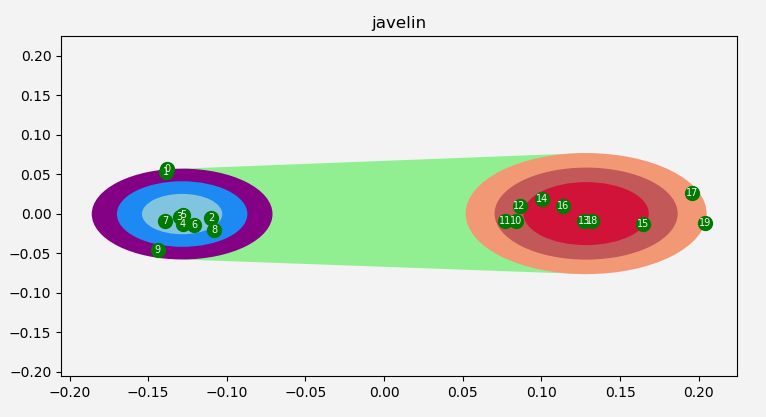
\includegraphics[width=\textwidth]{pictures/feedback_expert_cluster_example.png}
    \caption[Clusters formés par les données de l'expert]{Exemple de clusters formés à partir des données de l'expert (points verts). En bleu, le cluster des bons gestes, en rouge, le cluster des mauvais gestes pour le défaut appelé " Javelin ".}
    \label{fig:feedback_expert_cluster_example}
\end{figure}


Les limites de cette approche se situent dans l'impossibilité de corriger le problème si jamais deux clusters se superposent. La superposition des clusters implique que les différences entre les bons et mauvais gestes peuvent être plus ou moins floues, en fonction du degré de superposition. Cela implique que les données de l'expert ne sont pas suffisamment significatives par rapport au défaut observé, ou que les descripteurs observés ne sont pas significatifs par rapport au défaut. Une piste serait de vérifier la superposition ou non des deux clusters, et de supprimer automatiquement les points de données dont la distance au centroïde du cluster auquel ils sont assignés est la plus extrêmes, afin de réduire ou d'annuler la superposition des clusters.

Pour la visualisation des données de l'apprenant par rapport à celles de l'expert, une réduction de dimensionnalité des données est nécessaire lorsque celle-ci est supérieure à 2. Pour cette étape, une analyse en composantes principales (\textit{PCA}) est utilisé, afin d'obtenir la dimensionnalité voulue en sortie. Cette étape est réalisée juste avant l'affichage, afin d'effectuer tous les calculs sur les données non-modifiées. Un exemple de cet affichage est présent sur la Fig. \ref{fig:feedback_full_example}. On y voit un exemple avec quatre défauts identifiés, ainsi que les données de l'expert (cercles rouges et bleus). Cet affichage permet d'identifier dans quelle mesure le geste de l'apprenant correspond au geste cible : on remarque que pour les défauts " leaning " et " elbow move ", le centroïde de l'apprenant (en rouge) est compris dans le cluster des bons mouvements de l'expert. Par contre, pour les défauts " javelin " et " align arm ", les données de l'apprenant sont en moyenne plus proche du cluster de mauvais gestes. Ainsi, l'expert peut se baser sur ce retour visuel pour proposer des exercices permettant d'améliorer ces deux aspects du geste concernés.

Afin de proposer le(s) conseil(s) jugé(s) le(s) plus pertinent(s), le système doit être en mesure de fournir une indication quant à la présence plus ou moins forte des défauts identifiés. Pour répondre à ce besoin, une distance entre le centroïde des données de l'apprenant et les clusters expert est calculé. Soit $c_g$ le centroïde du clusters des bons gestes, $c_b$ le centroïde du clusters des mauvais gestes, et $c_a$ le centroïde des données de l'apprenant. On définit :
\[ A = y_{c_b} - y_{c_g} \]
\[ B = x_{c_b} - x_{c_g} \]
\[ C = (x_{c_g} * y_{c_b}) - (x_{c_b} * y_{c_g}) \]
La distance $D$ est défini comme il suit :
\[ D = \frac{A * x_{c_a}+ B * y_{c_a} + C}{\sqrt{A^2 + B^2}}\]

Cette distance correspond à la distance entre le centroïde des données de l'apprenant et le point de la droite reliant les centroïdes des deux clusters experts le plus proche. Elle se base sur l'hypothèse que si les données de l'apprenant se situent dans le trapézoïde (en vert sur les Fig. \ref{fig:feedback_full_example} et  \ref{fig:feedback_expert_cluster_example}) reliant les deux clusters de l'expert, le défaut est plus facilement corrigeable que s'il est en dehors de cette zone. Elle permet d'évaluer à quel point les descripteurs des données de l'apprenant sont éloignés de ceux de l'expert : plus elle est grande, plus l'apprenant est loin du geste de l'expert pour un défaut donné. Selon les cas d'utilisations, ce conseil peut être utilisé tel quel, ou l'expert peut se baser sur (i) la visualisation proposée par le système et/ou (ii) les conseils fournis par le système. Dans l'exemple montré dans la Figure \ref{fig:feedback_full_example}, on peut noter que le centroïde de l'apprenant, pour le défaut « \textit{align arm} », est situé en dehors des clusters et de l'espace situé entre ces clusters. Dans ce cas de figure, l'explication de cette distance peut être problématique. En effet, si les centroïde se situe dans l'alignement des clusters, bien qu'il soit en dehors des clusters et de la zone située entre eux, on peut supposer que le défaut est encore plus accentué chez l'apprenant. Cependant, lorsque le centroïde ne se situe pas dans cet alignement, il nous est pour l'instant impossible de donner une indication précise sur la nature du défaut de l'apprenant seulement à partir des données de mouvement ; ce point devra être travaillé dans le futur. Une piste serait de comparer la distance entre chaque descripteur extrait, afin de donner un retour sur l'aspect du geste étant le plus mauvais.
\afterpage{
\begin{landscape}
\begin{figure}
	\centering
    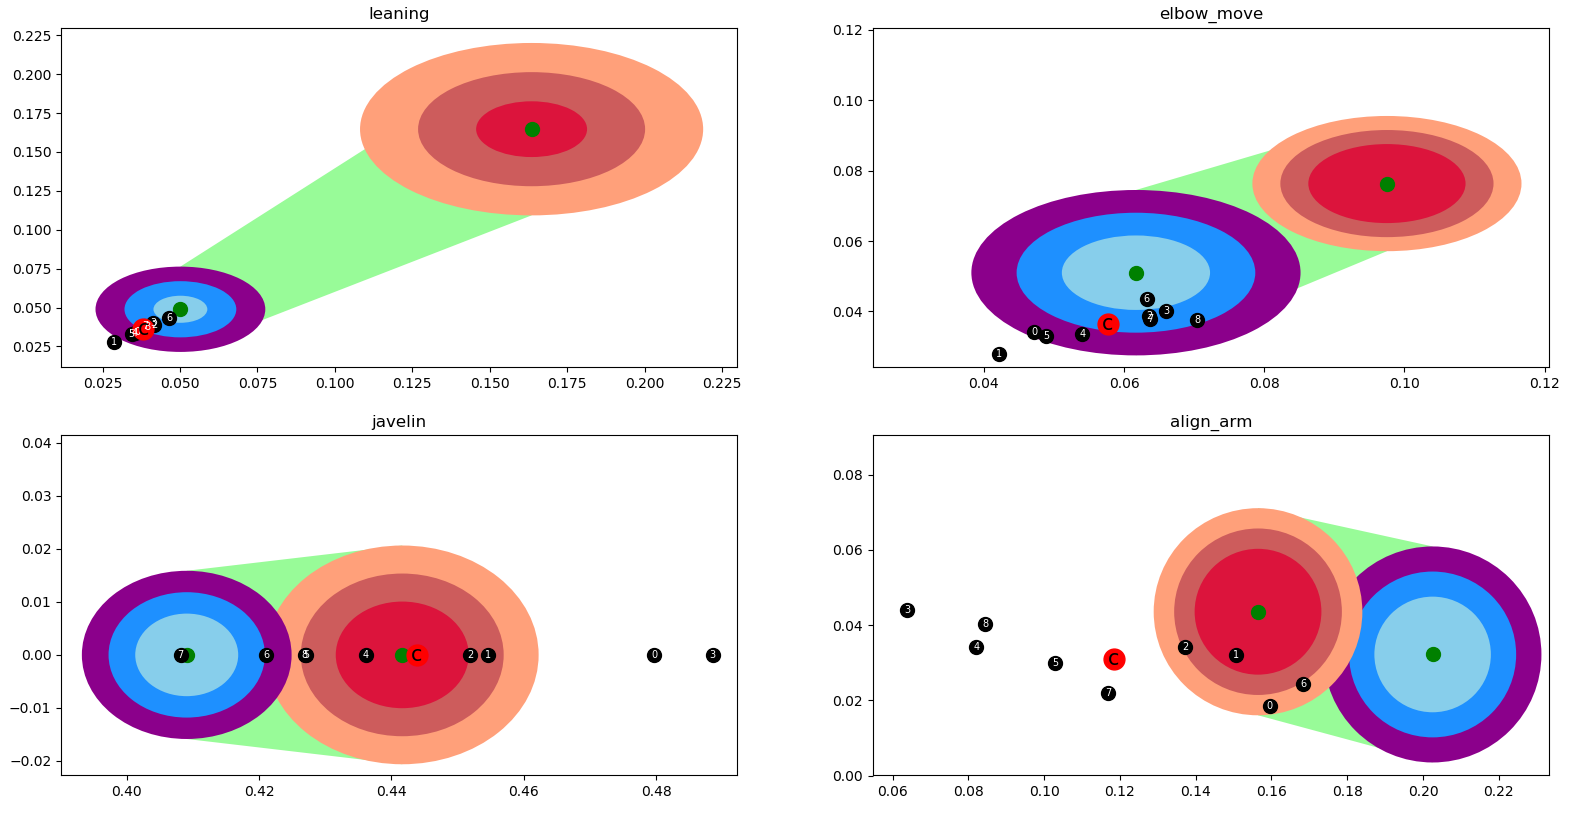
\includegraphics[width=23cm]{pictures/feedback_full_example.png}
    \caption[Feedback visuel proposé à l'expert]{Exemple de feedback visuel proposé à l'expert. Pour chaque défaut identifié (4 dans le cas présent), une visualisation des données de l'apprenant (points noirs) ainsi que du centroïde correspondant (points rouges) est affiché, afin de visualiser la distance de ces derniers par rapport aux données de l'expert pour un défaut identifié.}
    \label{fig:feedback_full_example}
\end{figure}
\end{landscape}}

\section{Résumé des contributions}
Dans cette partie, une chaine de traitement adaptée au Perception Neuron, pour l'analyse du mouvement capturé en situation d'apprentissage a été présentée. Les problèmes auxquels cette chaine de traitement propose des réponses sont (i) la modification de la taille des membres au cours du mouvement, (ii) les incohérences de positions des capteurs entre certaines frames. Plusieurs étapes de filtrage des données ont été présentées afin de palier ces problèmes. L'incohérence de positions des capteurs se traduisait par la présence de pics lors de l'extraction des vitesses. Ces pics ne correspondaient pas à la réalité du geste. Un filtre passe-bas a été appliqué, afin de compenser les artefacts du signal. Le problème de cette méthode est que les paramètres du filtre doivent être estimés (soit empiriquement, soit automatiquement) pour chaque signal, en fonction de ses caractéristiques propres, afin de ne pas trop " lisser " les valeurs réelles du signal.

Afin de ne garder que la partie utile du mouvement, un algorithme de segmentation a été présenté. L'algorithme de segmentation du mouvement utile permet de ne garder que les parties voulues du mouvement. Cet algorithme se base sur le maximum de la vitesse d'une articulation possédant les amplitudes et/ou variations du mouvement les plus importants, puis recherche un nombre prédéfini de minimums locaux les plus proches (à gauche et à droite). Il est possible de choisir le nombre de minimums locaux désirés, afin de garder une plus ou moins grande partie du signal original. Les limitations de cet algorithme se trouvent dans le postulat que le mouvement d'intérêt présente la vitesse la plus élevée.

Cette chaîne de traitement possède l'avantage d'être peu consommatrice de ressources dans le traitement des mouvements par rapport aux méthodes de la littérature, ce qui permet une utilisation en direct sur le terrain. En effet, le temps moyen de traitement d'un mouvement (allant du filtrage à l'extraction de données) est de cinq secondes. Cette étape de filtrage des données est cruciale, afin de pouvoir extraire des informations du mouvement qui seront cohérentes avec la réalité du geste.

Le système de retour à l'apprenant proposé dans cette partie permet d'obtenir une information visuelle de la performance de l'apprenant, par rapport à l'expert. À partir de données d'expert, contenant des bons mouvements et des mouvements présentant des défauts, et des données de l'apprenant, un affichage graphique permet de visualiser les différences entre le geste de l'expert et celui de l'apprenant. L'expert peut ensuite se baser sur ce retour afin d'ajuster ou non son jugement. Ce système permet d'analyser des modalités du gestes qui ne serait pas possible d'observer en temps normal, par exemple de par la nécessité d'observer trop de parties du corps à la fois, ou par l'occlusion de parties du corps résultant du mouvement lui-même.

Ce système a fait l'objet de plusieurs expérimentations, afin de vérifier son bon fonctionnement et sa capacité à fournir un retour à l'expert et à l'apprenant. Le prochain chapitre est consacré à ces expérimentations.